
The challenge of determining optimal build sites,technology mixes or supply routes 
for energy systems has seen a number of mixed-integer linear formulations proposed
\cite{hoffmann2024review}. To introduce and motivate modelling energy site locations
and technology choices using a CFLP framework we illustrate using a simplistic example. \par

\begin{figure}[H]
    \centering
    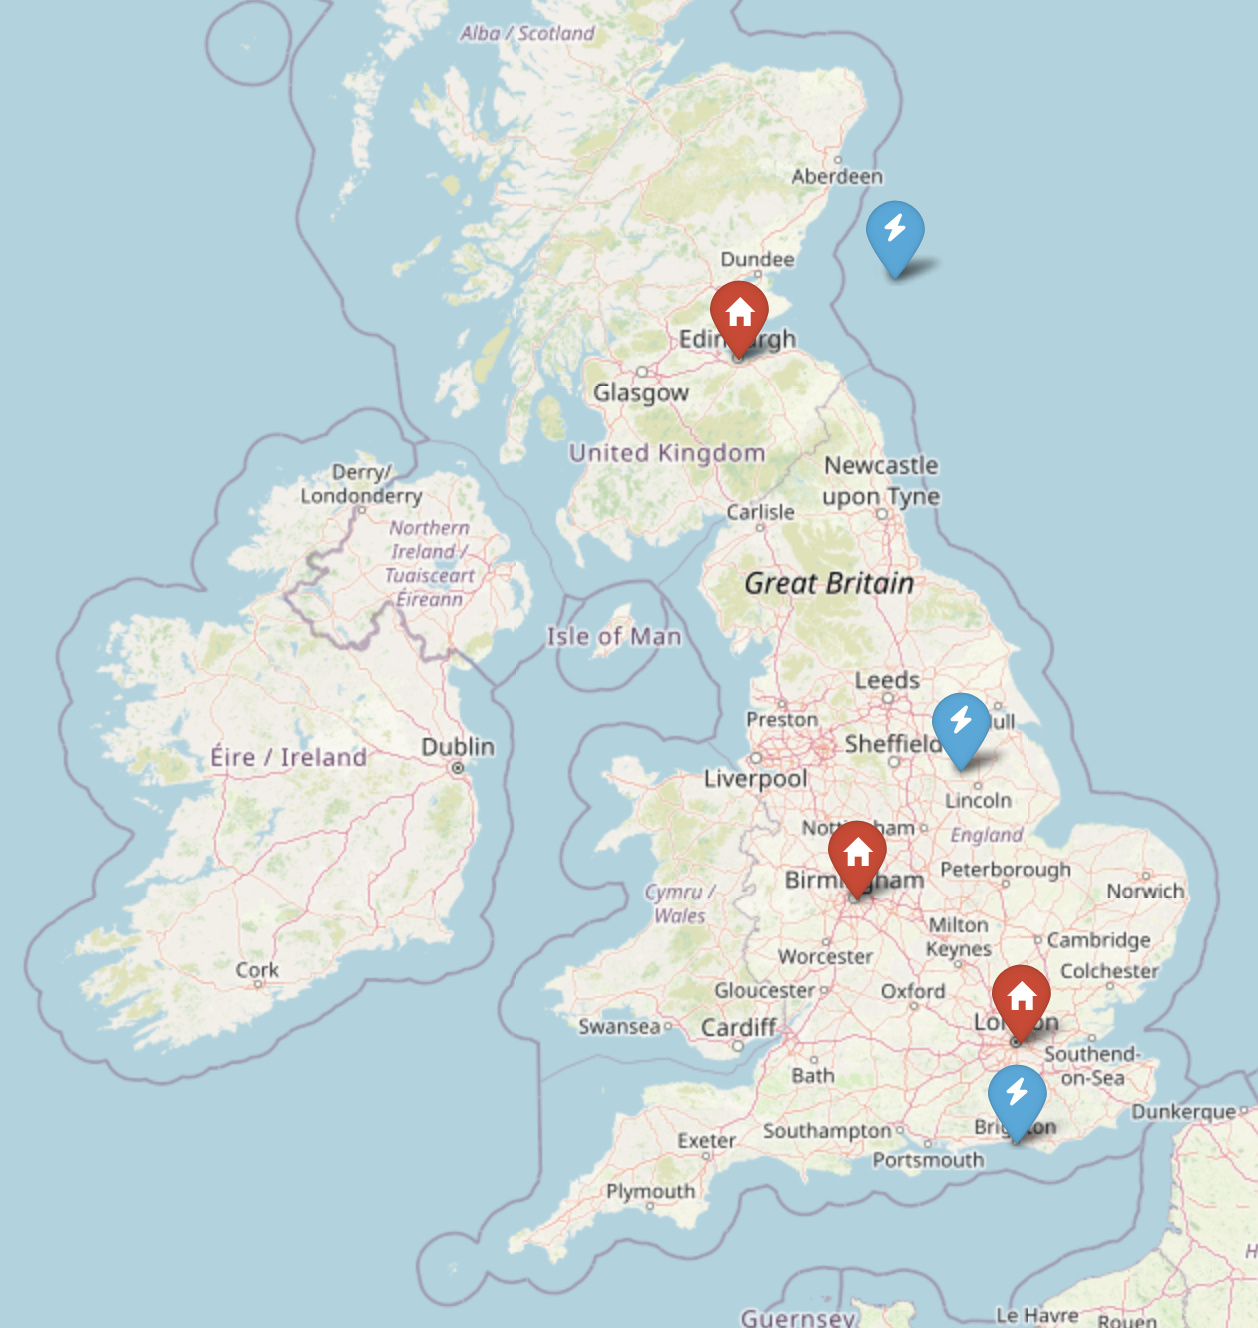
\includegraphics[width=0.4\textwidth]{figures/intro_example.png}
    \caption{Basic Energy Systems Problem}
    \label{fig:intro_plot}
\end{figure}


Figure \ref{fig:intro_plot} plots 3 potential renewable energy power plant sites marked with blue power
icons and 3 demand sites requiring power with red house markers. Each demand site has an associated energy
demand typically measured in MWh or GWh depending on the scope being considered, and each power plant
has an associated cost in supplying energy that can be measured in financial cost per GWh. Each supply site
also has its own associated maximum capacity it can supply. We derive estimates for these associated 
costs and capacities in Section \ref{sec:data_and_processing} when outlining the case study, but 
at this point it is sufficient to see
that if we wish to identify which set of renewable energy sites best meeets energy demands at the
lowest cost, then framing this as a CFLP is a natural choice. \par

However, energy systems need to optimise for varying demand over some time horizon.
Energy demands fluctuate, and depending on the application, time windows can be considered over hourly,
seasonal or annual time periods. Any analysis aiming to optimise this system should consider minimising 
cost to meet fluctuating demand, and this the CFLP does not consider. Similarly, supply costs can also vary
over time.
Therefore, we propose a modification to the CFLP that considers fluctuating demand, which in this report
is called the Energy Systems Location Problem (ESLP). Further modifications could have been considered, 
and these are discussed in Section \ref{sec:future_modifications}.\par

To setup the ESLP, we again consider supply and demand sets $S$ and $D$, again indexed by $s \in S$ and $d \in D$. 
We also add the set $T$ indexed by $t \in T$ to the problem, which represents the set of time points along which 
this problem is being considered. By $c_{s, d, t}$ we describe the cost incurred for supply site $s$ to supply demand 
site $d$ with a unit of demand at time $t$. As in the CFLP, $f_s$ denotes the cost associated with setting up site $s$.
Setup is assumed to have taken place initially (although cases where setup can occur at different times
could be a valuable modification for capital planning, see Section \ref{sec:future_modifications}).
$u_{s}$ denotes the maximum capacity of site $s$ through a single time period $t$ and $r_{d, t}$ denotes the demand required to be met at site 
d at time t. Our decision variables now are $x_{s, d, t} \in \mathbb{R}_{\geq 0}$ which describes the amount supplied by 
supply site $s$ to demand site $d$ at time $t$, and $y_s \in \mathbb{B}$ which indicates whether supply site $y$ is 
constructed or not. The ESLP problem is therefore:

\begin{subequations}\label{eq:ESLP}
    \begin{align}
    \text{ESLP: } \quad \quad \min \quad & \sum_{s \in S} f_s y_s + \sum_{s \in S}\sum_{d \in D}\sum_{t \in T} c_{s,d,t} x_{s,d, t} \label{eq:ESLP_obj}\\
    \text{subject to: } & \sum_{s \in S} x_{s,d,t} \geq r_{d,t} \quad \forall d \in D, \forall t \in T, \label{eq:ESLP_dem}\\
    & \sum_{d \in D} x_{s,d, t} \leq u_{s} y_s, \quad \forall s \in S, \forall t \in T, \label{eq:ESLP_cap}\\
    & y_s \in \{0, 1\}, \quad \forall s \in S,\label{eq:ESLP_y}\\
    & x_{s,d,t} \geq 0, \quad \forall s \in S, \forall d \in D, \forall t \in T.\label{eq:ESLP_x}
    \end{align}
\end{subequations}

\ref{eq:ESLP_obj} is the objective function to be minimised for the ESLP. \ref{eq:ESLP_dem} encodes the requirements that
at all points in time the demand at demand site d must be met. \ref{eq:ESLP_cap} says that at no points in time can a 
supply site exceed its capacity. \ref{eq:ESLP_x} and \ref{eq:ESLP_y} represent the integrality constraints.
